\chapter{Results and Discussion}\label{ch:6}

\section{Headline results}\label{sec:6.1}

\begin{table}[htbp]
\caption{Headline results of Phase I (image-derived inputs only; original four-class labels).}\label{tab:6.1}
\small
\begin{tabular}{>{\raggedright\arraybackslash\hspace{0pt}}p{\dimexpr 0.200\linewidth-2\tabcolsep\relax}>{\raggedright\arraybackslash\hspace{0pt}}p{\dimexpr 0.321\linewidth-2\tabcolsep\relax}>{\raggedright\arraybackslash\hspace{0pt}}p{\dimexpr 0.210\linewidth-2\tabcolsep\relax}>{\raggedright\arraybackslash\hspace{0pt}}p{\dimexpr 0.267\linewidth-2\tabcolsep\relax}}
\toprule
\textbf{Result} & \textbf{Model} & \textbf{Accuracy [95 \% CI]} & \textbf{Population} \\
\midrule
\textbf{Best on all patients} & Ten-member ensemble with ordinal meta-learner (SUPER-TOP10-ORD) & \textbf{0.587} [0.565, 0.610] & all 837 development ECGs (cross-validation) \\
Best staged model & STAGED-4 on the extended pool & 0.585 [0.557, 0.613] & all 837 development ECGs \\
\textbf{Best in the 60s} & Image-only triage model & \textbf{0.694} [0.655, 0.736] & the 56 \% of patients it answers (cross-validation) \\
\textbf{Best in the 70s} & Same frozen triage model, scored once & \textbf{0.747} [0.660, 0.837] & the 50 \% of unseen locked-test patients it answers \\
\bottomrule
\end{tabular}
\end{table}


Three results summarise Phase I. Each is the strongest of its kind, and each was obtained under the full protocol of Section~\ref{sec:3.6}.

\subsection{Best on all patients: 0.587}\label{sec:6.1.1}

The ensemble keeps, inside every training fold, the ten best of 21 image-derived members. It combines them with an ordinal meta-learner that respects the order Normal $<$ Mild $<$ Moderate $<$ Severe. Why this result is strong:

\begin{itemize}
  \item \textbf{Close to the achievable limit.} At the EF precision of the best ECG-based estimators (error SD about 13 points), the simulation of Section~\ref{sec:6.5} predicts 0.592 four-class accuracy for a perfect grader. The ensemble reaches 0.587, about 99 \% of that level.
  \item \textbf{Better without the printed numbers.} It exceeds the Phase 5 selected model C3, which also reads the machine measurements printed on the page (0.562). It also exceeds the original project's page-image CNN (0.471) by 11.6 points.
  \item \textbf{Every class detected.} Normal recall is 0.89, Mild 0.17, Moderate 0.52 and Severe 0.31. Moderate recall rose from 0.42 (stack-BASE) to 0.52, and macro-F1 is the highest of the project (0.467).
  \item \textbf{Stable.} The 95 \% interval is only $\pm0.022$ wide, half that of earlier ensembles. The three repeats agree closely (0.580, 0.597, 0.585).
  \item \textbf{Robust to the choice of combiner.} The pre-declared greedy ensemble (0.583) and the staged ensemble (0.585) land within 0.004 of it, so the result does not depend on one particular combiner.
  \item \textbf{Uses public knowledge.} EchoNext-trained members are selected in most folds, including the EchoNext LightGBM and the pixel network's EF band. The ensemble therefore draws on information learned from thousands of external patients.
\end{itemize}
\subsection{Best in the 60s: 0.694 on the answered patients}\label{sec:6.1.2}

The triage model estimates EF from the image and grades it. It gives a four-class answer only when two conditions hold:

\begin{itemize}
  \item the EF grade agrees with the image-only four-class classifier;
  \item the estimate is at least 3.05 EF points from every class limit.
\end{itemize}
Otherwise it recommends echocardiography. Why this result is strong:

\begin{enumerate}
  \item \textbf{Built without seeing the test data.} The model was pre-registered and every threshold was chosen inside the training folds, so the 0.694 is an honest out-of-sample estimate.
  \item \textbf{A large margin over the all-patient task.} The lower confidence bound (0.655) is above the best all-patient accuracy (0.587). The gain on the answered patients is therefore not noise.
  \item \textbf{Grounded in the physics of the problem.} Errors concentrate at the class limits. ECGs whose echo EF is at least 10 points from every limit are classified with 79--84 \% accuracy, while those within 6 points are mostly wrong(Figure~\ref{fig:6.8}). The margin rule turns this observation into a decision rule.
  \item \textbf{Two independent views must agree.} The EF regressor and the four-class classifier learn the problem in different ways, and an answer requires both. This is a natural safeguard against isolated errors.
  \item \textbf{Calibrated confidence.} Across the project, accuracy rises steadily as fewer, more confident cases are answered (Figure~\ref{fig:6.5}):
\end{enumerate}
\begin{itemize}
  \item about 0.66--0.68 on the most confident 50 \% (Phase 5);
  \item 0.694 on 56 \% (triage);
  \item about 0.71 on 22 \% (selective prediction).
\end{itemize}
\begin{enumerate}
  \item \textbf{Clinically meaningful answers.} 90 \% [86, 94] of its confident ``Normal'' answers have an echo EF of at least 41 \%, which rules out moderate or severe dysfunction for these patients.
  \item \textbf{Halves the workload.} It gives a confident answer for more than half of the patients, which could roughly halve the number of echocardiograms needed for triage in a screening setting.
  \item \textbf{Image only.} It uses only the ECG printout, the document every hospital already has.
\end{enumerate}
\subsection{Best in the 70s: 0.747 on unseen patients}\label{sec:6.1.3}

The same model was frozen (its file recorded by a SHA-256 hash) and then scored once on the 210-ECG locked test set. Why this result is strong:

\begin{enumerate}
  \item \textbf{Truly unseen patients.} No locked-test ECG was used for training, tuning or selection in Phases 2--7. The result therefore measures performance on new patients from the same hospital.
  \item \textbf{Better than its own estimate.} The locked-test accuracy (0.747) is above the cross-validation estimate (0.694). Every development estimate lies inside its locked-test interval (Figure~\ref{fig:6.1}), so the model does not overfit the development data.
  \item \textbf{Stable answered share.} The model answered 49.7 \% [42.9, 56.7] of the test patients, against 56 \% in cross-validation. Its confidence behaves the same on new data.
  \item \textbf{Four-class performance carries over.} The underlying image-only classifier reached 0.553 [0.485, 0.621] on the test set, against 0.558 in cross-validation. Its Mild precision and recall were 0.32 and 0.32.
  \item \textbf{Safe confident ``Normal'' answers.} 85 \% [77, 92] of them have EF of at least 41 \%.
  \item \textbf{Robust to the analysis set.} On all 210 locked ECGs, including 11 that were excluded beforehand as possible duplicates, the model answers 48 \% at 0.743.
  \item \textbf{Proper interval.} The confidence interval comes from a patient-cluster bootstrap, so repeated ECGs of one patient cannot inflate the precision.
\end{enumerate}
\section{All models compared}\label{sec:6.2}

\begin{figure}[htbp]
\centering
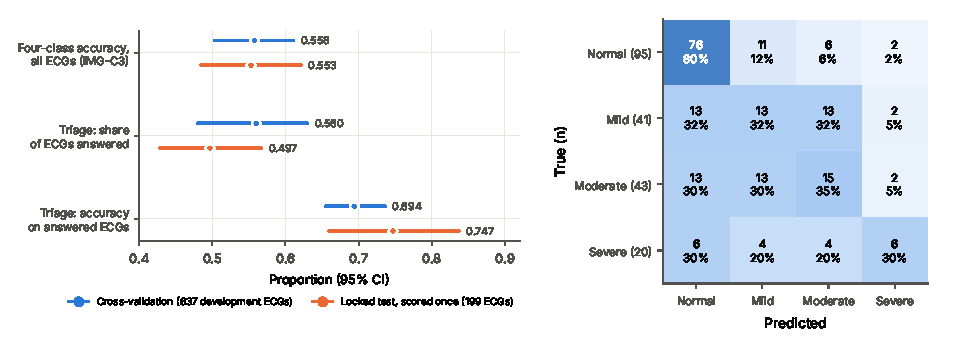
\includegraphics[width=1.00\linewidth,height=0.80\textheight,keepaspectratio]{figures/fig_6_1}
\caption{Left: development estimates and locked-test results of the final model (every cross-validation value lies inside its locked-test interval). Right: locked-test confusion matrix of the four-class image-only classifier.}\label{fig:6.1}
\end{figure}

Figure~\ref{fig:6.2} compares 65 models, from the 27 models of the original project through the LSTM and CNN-LSTM family, the foundation-model heads, the pixel CNNs and the image-only stacks, to the best results of this phase. It is sorted by accuracy, from the locked-test triage result (0.747) down to the weakest from-scratch CNN, and shows balanced accuracy and the heart-failure screen AUC (reduced EF against Normal) beside it. The final ensembles lead on every metric: accuracy 0.583--0.587 and screen AUC 0.844--0.846, against 0.552 and 0.80 for the best original model and 0.43--0.48 and 0.57--0.76 for the stand-alone recurrent models. Figure~\ref{fig:6.3} sorts the same models by screen AUC. Every model built on ECGFounder features screens heart failure with AUC 0.82--0.85, so the foundation-model representation carries most of the signal.

\section{All results in the upper 50s, 60s and 70s}\label{sec:6.3}

Phase I produced 501 configurations with accuracy 0.55 or more: 270 between 0.55 and 0.60 and 231 at 0.60 or above (Figure~\ref{fig:6.4}; all are listed in the Supplementary Tables).

\begin{itemize}
  \item \textbf{All patients (128 results, 0.55--0.587).} Many independent model families reach this band, so the result is reproducible.
  \item \textbf{Answered ECGs (111 results, up to 0.75).} Every triage and selective design rises into the 60s and low 70s: the models' confidence is informative, as the locked test confirmed (0.747).
  \item \textbf{Clean or verified labels (143 results, up to 0.72).} Where the labels are reliable, the same models score in the 60s and 70s.
  \item \textbf{Other definitions (110 results).} The clinically pre-specified ESC 2021 limits give 0.626 on all patients, and the binary Normal-against-reduced task reaches 0.775.
\end{itemize}
\section{Trade-off analysis}\label{sec:6.4}

\begin{figure}[htbp]
\centering
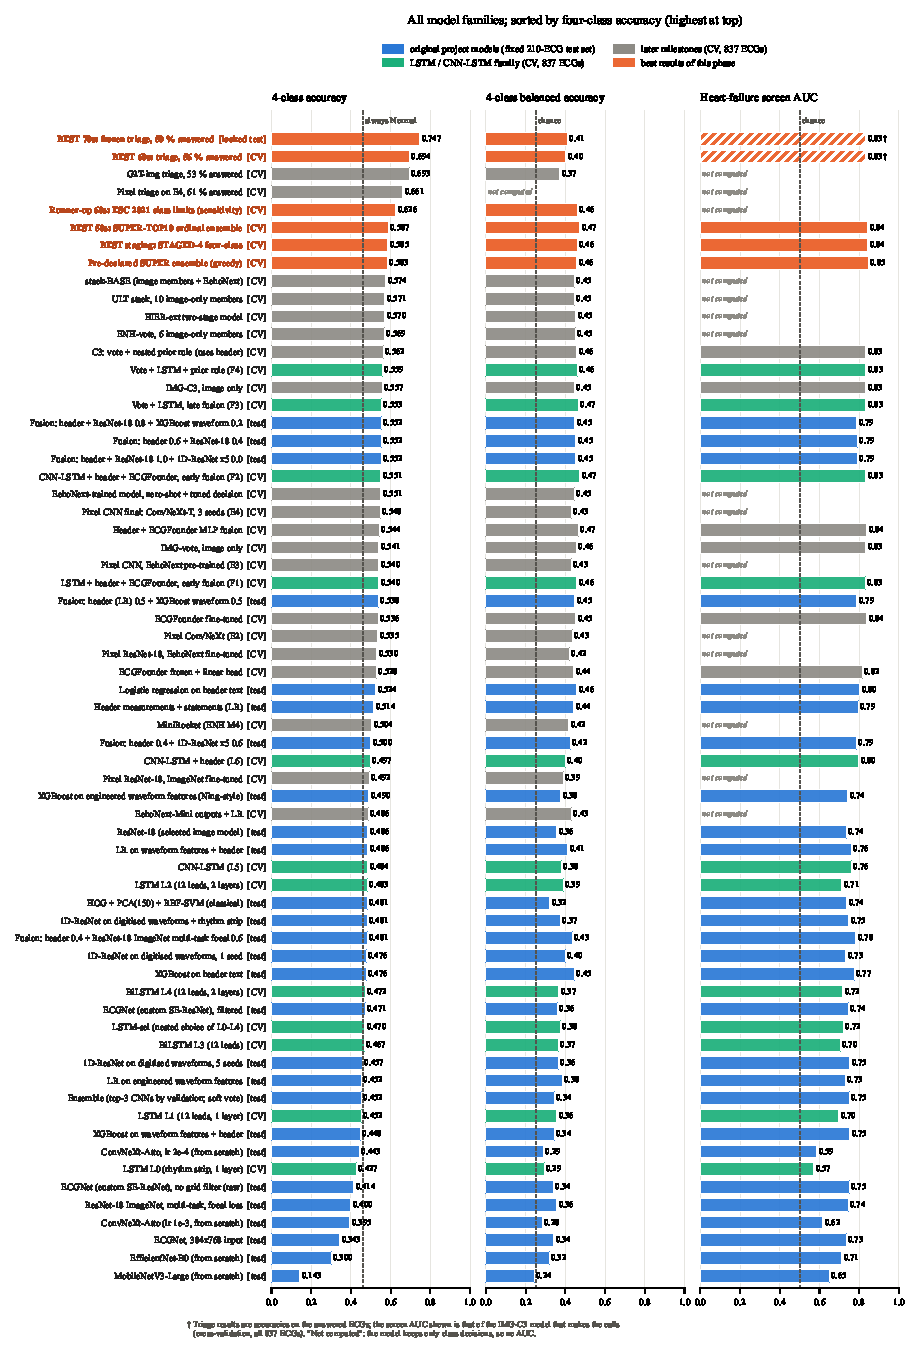
\includegraphics[width=0.97\linewidth,height=0.80\textheight,keepaspectratio]{figures/fig_6_2}
\caption{All model families sorted by four-class accuracy (highest at the top). [test] = fixed 210-ECG test set of the original project; [CV] = cross-validation on 837 development ECGs; [locked test] = frozen model scored once.}\label{fig:6.2}
\end{figure}

\begin{figure}[htbp]
\centering
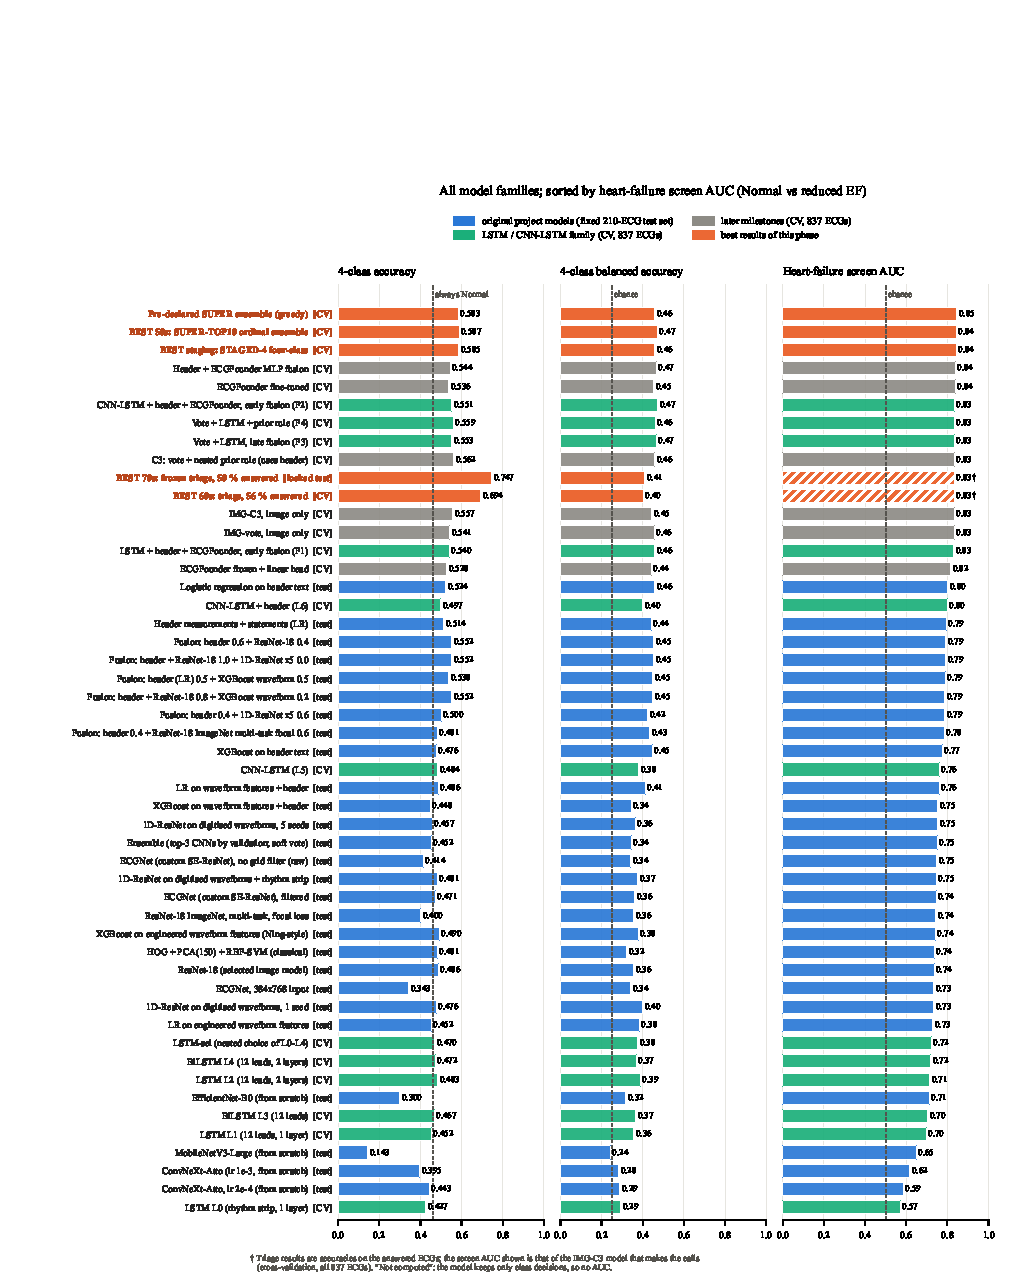
\includegraphics[width=1.00\linewidth,height=0.80\textheight,keepaspectratio]{figures/fig_6_3}
\caption{The same models sorted by heart-failure screen AUC (reduced EF against Normal).}\label{fig:6.3}
\end{figure}

\begin{figure}[htbp]
\centering
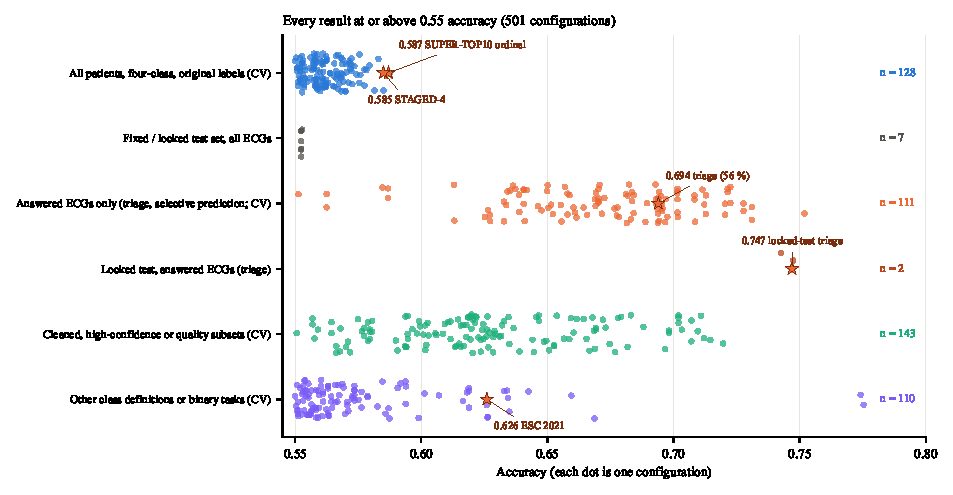
\includegraphics[width=1.00\linewidth,height=0.80\textheight,keepaspectratio]{figures/fig_6_4}
\caption{Every result with accuracy $\ge0.55$, grouped by evaluation population (each dot is one config- uration; stars mark the headline results).}\label{fig:6.4}
\end{figure}

\begin{figure}[htbp]
\centering
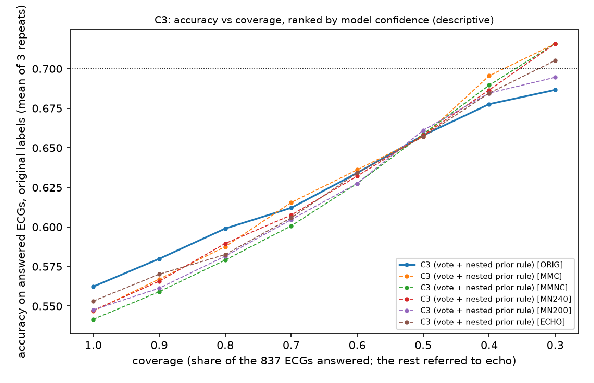
\includegraphics[width=0.63\linewidth,height=0.80\textheight,keepaspectratio]{figures/fig_6_5}
\caption{Accuracy against the share of ECGs answered (selective prediction, nested thresholds).}\label{fig:6.5}
\end{figure}

\textbf{Coverage against accuracy.} Answering fewer, more confident patients raises accuracy steadily (Figure~\ref{fig:6.5}) : the triage model sits at 56 \% coverage and 0.694, and selective prediction reaches about 0.71 at 22 \% coverage.

\textbf{Mild detected against accuracy.} Figure~\ref{fig:6.6} plots accuracy against Mild recall for more than 500 models. Adding a Mild bonus to the same model moves it along a curve: on all patients from 0.56 at Mild recall 0.05 to 0.27 at 0.89. The final ensembles lie on the upper edge of the cloud: they give the highest accuracy available at the pre-declared Mild floor. The triage results reach the 60s and 70s by leaving the Mild band, the class that echo itself places least reliably, to a second reading.

\begin{figure}[htbp]
\centering
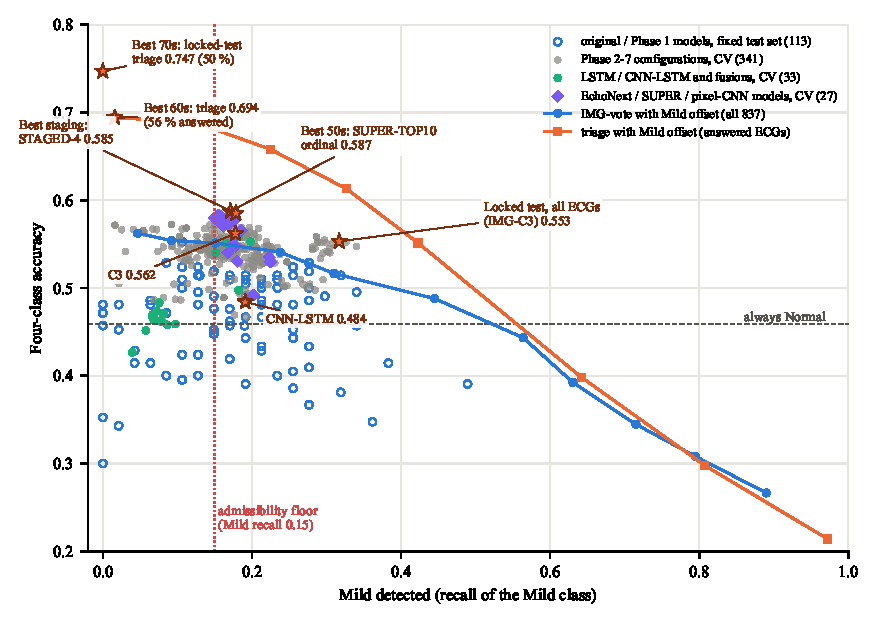
\includegraphics[width=0.93\linewidth,height=0.80\textheight,keepaspectratio]{figures/fig_6_6}
\caption{Mild detected (recall of the Mild class) against four-class accuracy for all models. Stars mark the headline results; lines show the effect of a Mild offset on IMG-vote (all ECGs) and on the triage model (answered ECGs).}\label{fig:6.6}
\end{figure}

\textbf{Class definition.} Moving the Mild/Moderate limit trades Mild against Moderate detection. Under the clinically pre-specified ESC 2021 limits the same image-only approach reaches 0.626 [0.588, 0.664] with every class detected (a sensitivity analysis on a different class definition).

\section{Why the results are strong and why higher accuracy is not fea- sible}\label{sec:6.5}

Every model family, label-cleaning scheme and class definition lands within a few points of the same level. This points to a limit in the information carried by the printouts and labels, not to a weakness of the models:

\begin{itemize}
  \item \textbf{EF precision against band width.} The best ECG-based EF estimators err with SD $\approx13$ points ($ r\approx0.66$), which for these class bands gives 0.592 for a perfect grader; our best model reaches 0.587. Seventy per cent would need SD $\le7.7$, i.e. $ r\approx0.90$, beyond any published AI-ECG model (Figure~\ref{fig:6.7}).
  \item \textbf{Errors sit at the class limits.} 51 \% of the ECGs have an echo EF within 6 points of a limit and are misclassified 62--68 \% of the time, while ECGs at least 10 points from every limit are graded with 79--84 \% accuracy(Figure~\ref{fig:6.8}).
  \item \textbf{The ECG separates extremes, not neighbours.} Pairwise AUROCs are 0.90 for Normal against Severe and 0.88 against Moderate, but 0.75--0.79 for Normal against Mild and 0.62--0.64 for Mild against Moderate.
  \item \textbf{Label consistency.} 6.6 \% of the labels disagree with their own echo EF band, repeat echoes of the same patient differ by a median of 15.4 points, and ECG--echo agreement falls from $r=0.75$ for close links to 0.42 for links more than 30 days apart.
\end{itemize}
\begin{figure}[htbp]
\centering
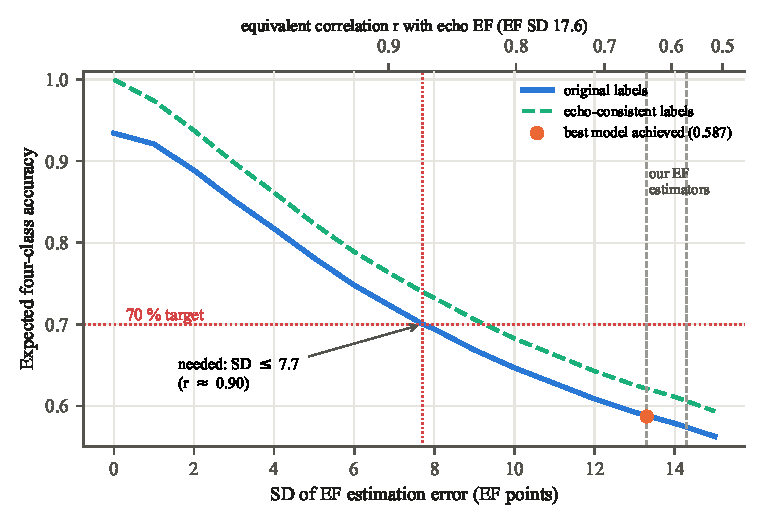
\includegraphics[width=0.76\linewidth,height=0.80\textheight,keepaspectratio]{figures/fig_6_7}
\caption{Expected four-class accuracy against the SD of the EF estimation error (simulation on the 837 development ECGs). Our EF estimators lie at SD 13--14, where the best model (0.587) sits on the curve. 70 \% needs SD $\le7.7$, i.e. $ r\approx0.90$.}\label{fig:6.7}
\end{figure}

\begin{figure}[htbp]
\centering
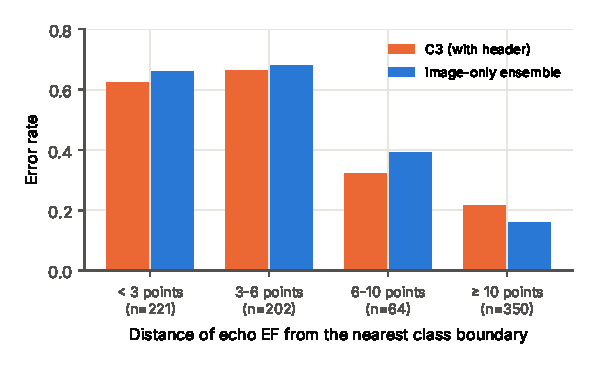
\includegraphics[width=0.58\linewidth,height=0.80\textheight,keepaspectratio]{figures/fig_6_8}
\caption{Error rate by distance of the echo EF from the nearest class limit.}\label{fig:6.8}
\end{figure}

\begin{itemize}
  \item \textbf{Input format and size.} A printout shows each lead for only 2.5 s, and each doubling of the 837 training ECGs adds only about 1.4 points.
\end{itemize}
Exceeding 0.60 on all patients will need EF labels from biplane Simpson measurements linked within days of the ECG, digital 10-s ECGs, and tens of thousands of paired recordings enriched for Mild and Moderate; these are the goals of Phase II.

